\documentclass{article}
\usepackage[preprint]{neurips_2022}


\usepackage[utf8]{inputenc} 
\usepackage[T1]{fontenc}  
\usepackage{hyperref} 
\usepackage{url}           
\usepackage{booktabs}    
\usepackage{amsfonts}       
\usepackage{nicefrac}       
\usepackage{microtype}      
\usepackage{xcolor}    
\usepackage{graphicx}
\usepackage{booktabs}





\title{Estimation of Electronic Band Gap Energy Using Machine Learning}


\author{
  Sagar Prakash Barad\\
  NISER Bhubaneswar\\
  \texttt{sagar.barad@niser.ac.in} \\
  \And
  Sajag Kumar\\
  NISER Bhubaneswar\\
  \texttt{sajag.kumar@niser.ac.in} \\
}


\begin{document}


\maketitle


\begin{abstract}
Our aim is to build a machine learning model that can estimate the electronic band gap energy of any material given its properties. Determination of band gap energy is crucial in determining many properties of a material (for example, determining whether it is a metal) and its potential applications (in electronic and optoelectronic devices). There are numerical methods available for computing band gap energy but they tend to be computationally very expensive and are limited in accuracy and size. A machine learning based model that can predict the band gap energy of materials quickly, given properties of materials that are easily determined experimentally, would be a much better alternative to traditional density functional theory based methods. We have built classification, regression and clustering algorithms to achieve this goal. We also tried ensemble methods for achieving higher accuracy but failed. The accuracy of all the classification algorithms is $>70\%$, with all of them performing better than random guessing. The $R^2$ for all the regression algorithms is $>0.72$. The clustering algorithm gave a reasonable number of clusters for future applications. 
\end{abstract}


\section{Introduction}

The energy of electrons in materials can not be arbitrary. Electrons are allowed to have certain special energy values. A band is a set of closely spaced energy values that an electron can occupy. Band gap is the difference between the energies of two different bands. In our case when we talk about band gap energy (or simply the band gap) we mean the difference between the energies of the valence and the conduction band. The conduction band consists of allowed energy values at which the electrons of the material conduct electricity. While the valence band is the set of allowed energies that the outermost electrons of the atoms of the material occupy. The valence band and the conduction band may overlap (band gap being zero) in which case the material is a metal, or they may be a little apart (small band gap) in which case the material is a semiconductor, or they may be far from each other (in which case the material is an insulator). Determination of band gap energy is of utmost importance for various reasons. For example, it tells us how much energy the electrons of a semiconductor are to be provided before the semiconductor starts conducting. The band gap energy also plays an important role in determining the potential of a material to find applications in various (electronic and optoelectronic) devices. \par
Recently there has been a dramatic increase in applications of machine learning in advancing material science. The bulk of the work is around predicting different material properties which involve energy calculations Carleo et al. [10]. Naturally a lot of work has been done around predicting band gap of materials. Most of the efforts have been directed to predicting the band gap of special class of materials for example, Olsthroon et al. [3] built ML models to predict the band gap of `large organic crystals' while Gao et al. [4] do it for `monolayer transition metal chalcogenide', the types of materials are in quotes to emphasise the narrow scope of these models. Even the more general attempts such as Zhang et al. [1] and Zhuo et al. [9] are designed for a special class of materials, 2D materials and inorganic solids respectively. While being able to predict the band gap of special types of material is good, these specialised models do not have to learn to predict the band gap from scratch because of their specificity they already have some ideas about the possible range of band gaps of the materials that they will see and they predict a value in this range, it would be much better if we can predict the band gap using only elementary properties of the material. This way we can also predict a lot of properties of the material. For example, if the band gap of a newly synthesised material is predicted to be zero, we immediately know it is a metal, without doing any further analysis. We attempt to build a general machine learning model that can estimate the electronic band gap of materials on the basis of elementary properties of the materials. In the following sections we present a brief review of some related works which made us believe that such a model can indeed be built. We also present some results of the various experiments we performed towards realising our goal. In the end we discuss the potential applications of deep learning in solving this problem.

\section{Related Works}

Zhang et al. [1] is the paper that we follow for most of our work. They build four types (support vector regression, gradient boosted decision trees, random forest and multi-layer perceptron) of ML models to predict the band gap of 2D materials. It can be seen in the ML for materials literature that Gradient boosted decision trees (GBDTs) and random forests (RFs) are more effective in learning material properties. This trend is also seen in this work, while GBDTs and RFs have an $R^2$ value of $0.92$ and $0.90$ respectively, SVR and MLP have an $R^2$ value of $0.75$ and $0.72$ respectively. Where $R^2$ is the explained variance.
where, the sum is over the test set, $y^{i}_{t}$ is the true band gap of the i-th test example, $\bar{y}^{i}_{p}$ is the average value of $y^{i}_{t}$ and $\hat{y}^{i}_{p}$ is the prediction of the model. The above stats are for the models trained on an eight-dimensional feature space. With the eight features being elementary properties of the materials obtained from the computational 2D materials database. In addition to this they also show that the introduction of a new feature, the band gap value of materials without the effect of spin orbit coupling (\emph{Gap\_nosoc}), leads to an increased accuracy for all the models. The \emph{Gap\_nosoc} feature value is calculated using traditional numerical methods ignoring complicated interaction terms. This shows that predicting band gap becomes much easier if it is known to lie in a certain range. More details about the dataset and the implemented algorithms is present in section \ref{sec:ml} and section \ref{sec:data}.\par

Kauwe et al. [7] perform ensemble learning to achieve greater accuracy than the baseline support vector regression. A special aspect of this paper is using multiple datasets for training the ML model. Their dataset is a mixture from \emph{the materials project}, \emph{AFLOW} and actual experimental data. They retain the heterogeneity of the combined dataset i.e. they do not throw out examples that have missing features. This is in striking contrast to what we said during the proposal, where we wanted to come up with a consistent classification scheme for different types of materials, which essentially means getting rid of the heterogeneity led to by combining different datasets. Three ensembling schemes have been implemented and compared with the baseline of just a support vector regressor (SVR). In our work we will follow a scheme similar to the first scheme presented in this paper in which predictions from three ML models, SVR, gradient boosting regressor (GBR) and random forest regressor (RFR) are fed as feature vector to a meta-learner (in this case a support vector regressor) which outputs the final prediction. The other two schemes achieve higher accuracy over the baseline but they use DFT based calculations as one of the feature values for the meta-learner. The ML models used for band gap prediction in this case are composition based, they do not predict the band gap on the basis of material properties but rather on the basis of their composition. \par
We also took inspirations from a couple of CS229 projects, Rosen et al. [5] and Hayee et al. [6]. None of them made a model for a specific class of materials. Their models are quite general. Hayee et al. [6] used $75$ features to train their ML models (RF, MLP, Ada Boosting and ordinary least square regression) with $2067$ samples in the dataset. They did not get very good results, with the best performing model ada boosting with $R^2 = 0.7$ on the test set clearly overfitting the training set with $R^2 = 1.0$. Rosen et al. [5] used only the position of atoms in the unit cell of the material to predict band gap. This required them to use an encoding scheme, the one-hot representation of constituent elements turned out to be the best among all the encoding schemes tested by them. Their model has two components a classifier (classifies metals and non-metals) and regressor (for the band gap prediction), while the one-hot representation of constituent elements encoding scheme worked well for both the classifier and the regressor, some of the encodings tested worked well only in one of the examples indicating that different encoding schemes allows the model to learn different aspects of the material. 

\section{Dataset}
\label{sec:data}

\begin{figure}
	\centering
	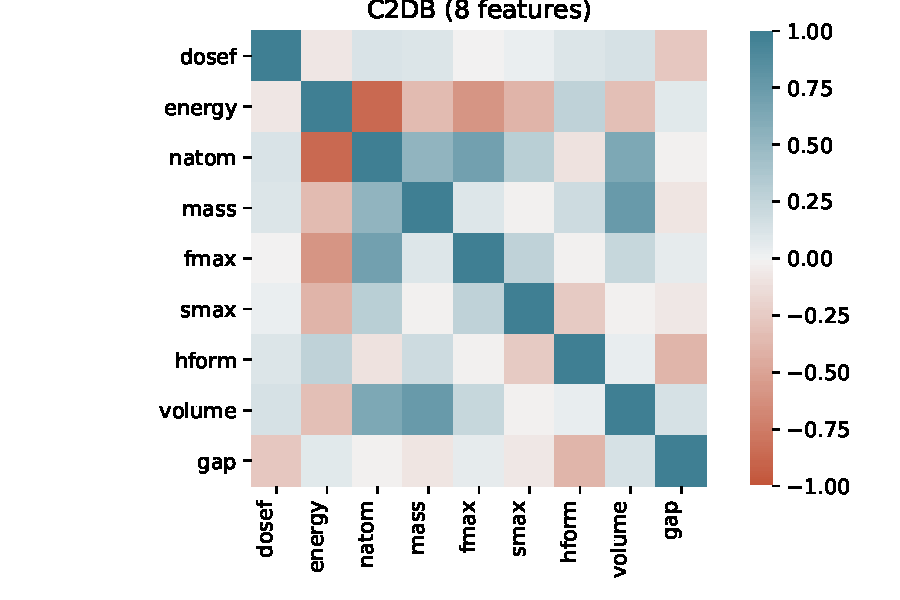
\includegraphics[width = 0.3\textwidth]{figures/c_8}
	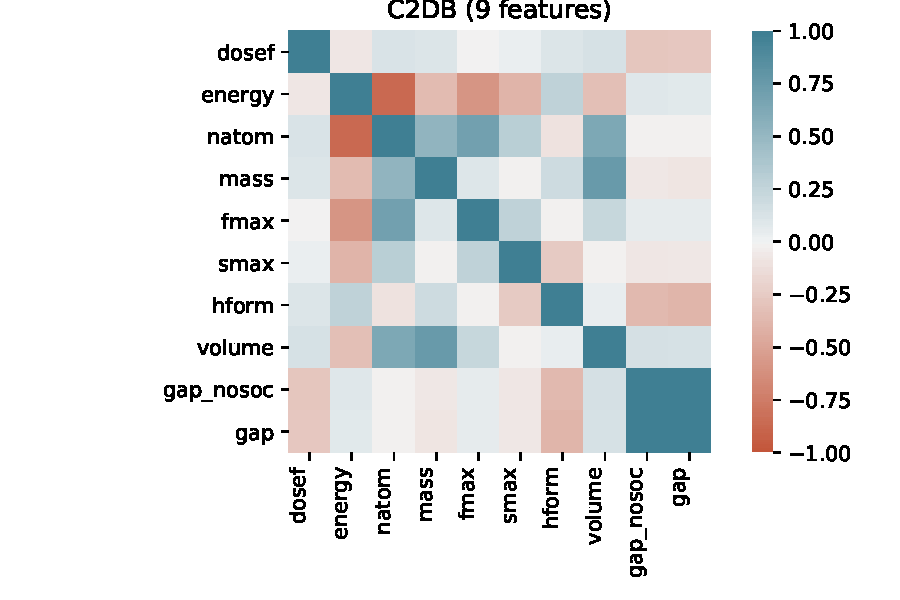
\includegraphics[width = 0.3\textwidth]{figures/c_9}
	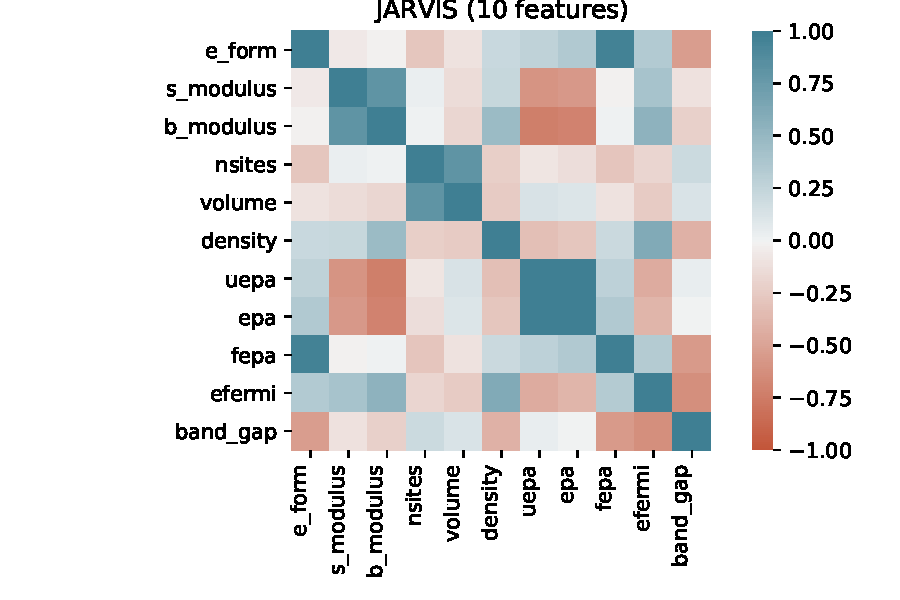
\includegraphics[width = 0.3\textwidth]{figures/j_10}
	\caption{Correlation matrix for C2DB and JARVIS. It is clear from the correlation matrix of nine dimensional C2DB dataset that \emph{gap} and \emph{gap\_nosoc} are very strongly correlated. \emph{uepa} and \emph{epa} are strongly correlated by dropping either of them did not improve the accuracy of the ML models trained on JARVIS. The correlation matrices are computed using spearman correlation coefficient following Zhang et al. [1].}
	\label{fig:c2db_data}
\end{figure}

We have used the following datasets
\begin{enumerate}

	\item \href{https://cmr.fysik.dtu.dk/c2db/c2db.html}{Computational 2D Materials Database (C2DB)} Choudhart et al. [11], we used the dataset used by Zhang et al. [1] which they uploaded along with their paper. Two datasets with eight and nine features were used by Zhang et al. [1], the correlation matrix for the dataset is shown in figure \ref{fig:c2db_data}. The eight (nine) dimensional dataset is present as .csv file with 3129 rows and 8 (9) columns respectively, 
	\item \href{https://jarvis.nist.gov/}{Joint Automated Repository for Various Integrated Simulations (JARVIS)} Haastrup et al. [12], we scrapped this dataset from \href{https://hackingmaterials.lbl.gov/matminer/}{matminer} REST API. The dataset we got had JARVIS ID for all the materials which was then referenced to scrape feature values of each, using the JARVIS REST API. The correlation matrix for the ten dimensional JARVIS dataset is shown in figure \ref{fig:c2db_data}. The JARVIS dataset is present as .csv file with 6590 rows and 10 columns.

\end{enumerate}

\section{Machine Learning Algorithms and Experiments}
\label{sec:ml}

\begin{figure}
	\centering
	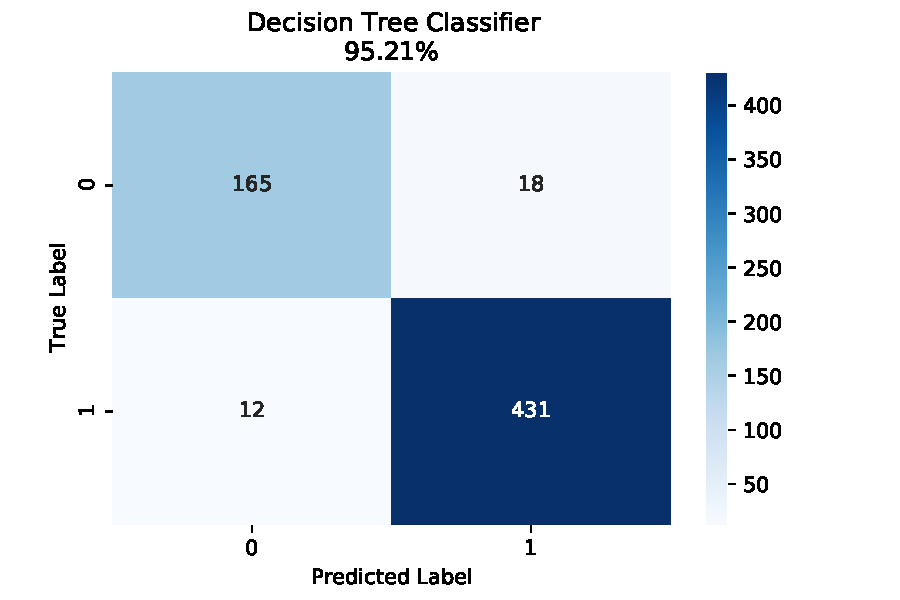
\includegraphics[width = 0.23\textwidth]{figures/c_dtc}
	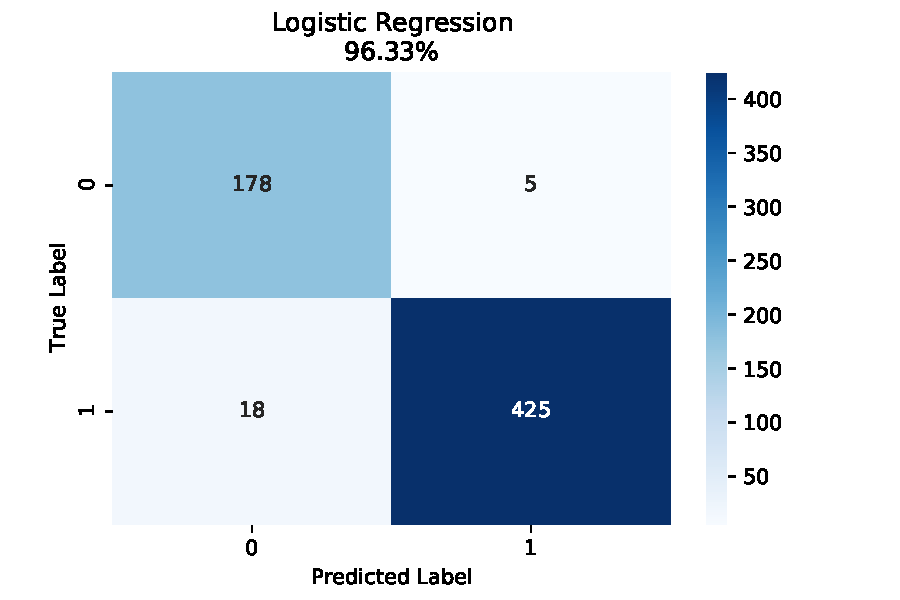
\includegraphics[width = 0.23\textwidth]{figures/c_lr}
	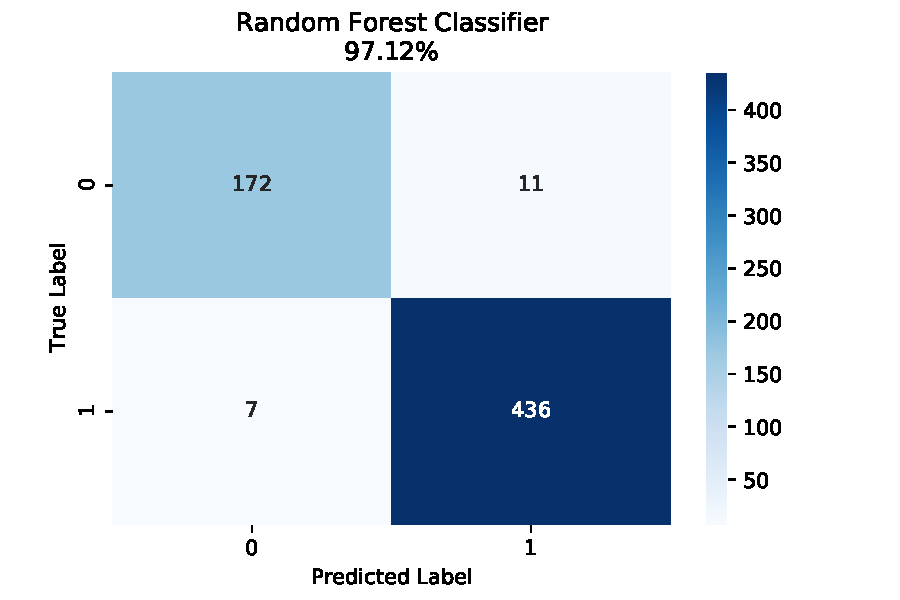
\includegraphics[width = 0.23\textwidth]{figures/c_rfc}
	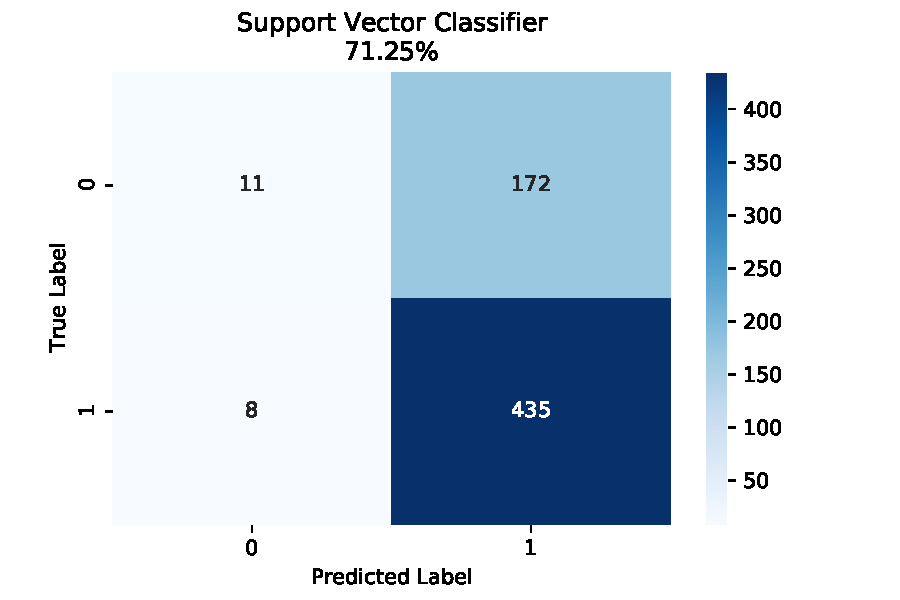
\includegraphics[width = 0.23\textwidth]{figures/c_svc}
	\caption{Confusion matrices for different classification algorithms trained on the C2DB dataset.}
	\label{fig:c}
\end{figure}

\begin{figure}
	\centering
	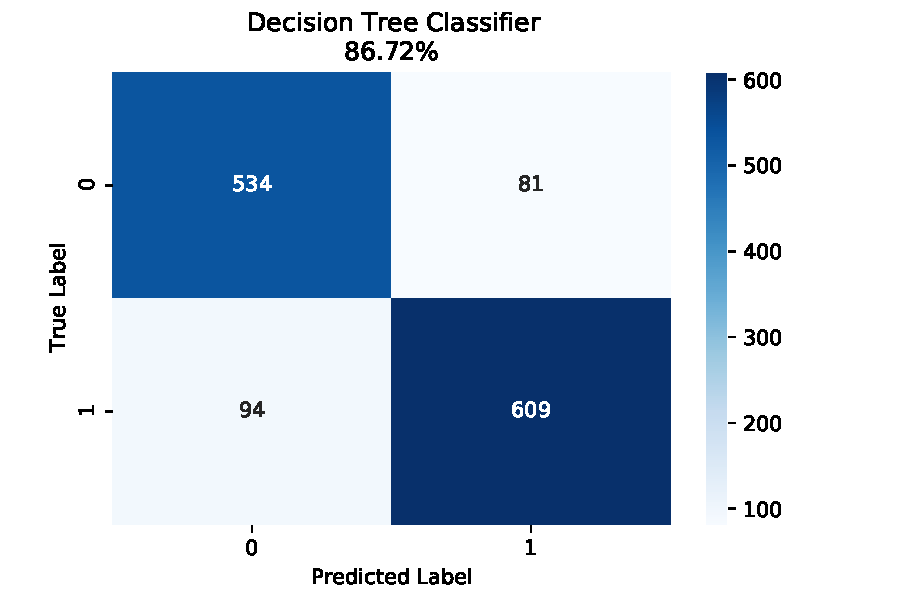
\includegraphics[width = 0.23\textwidth]{figures/j_dtc}
	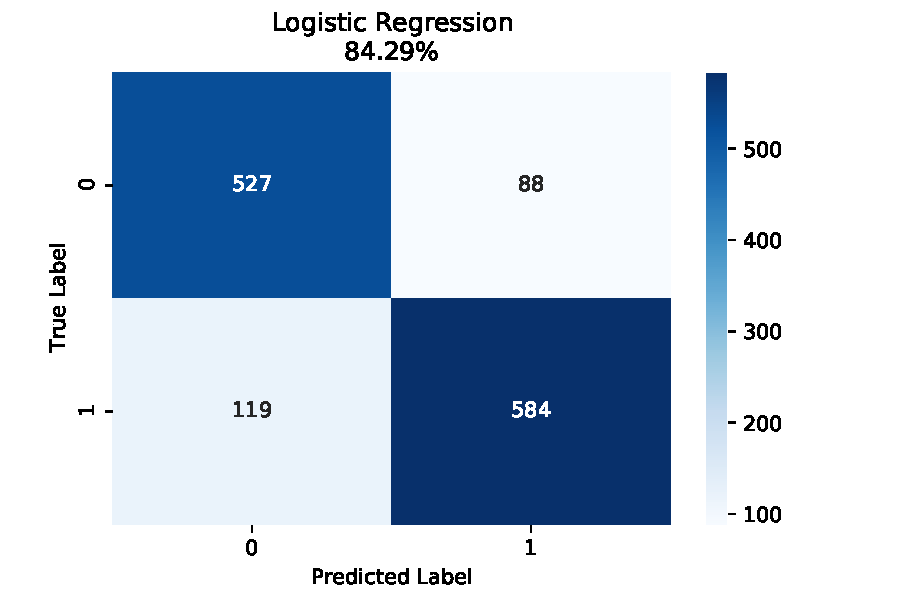
\includegraphics[width = 0.23\textwidth]{figures/j_lr}
	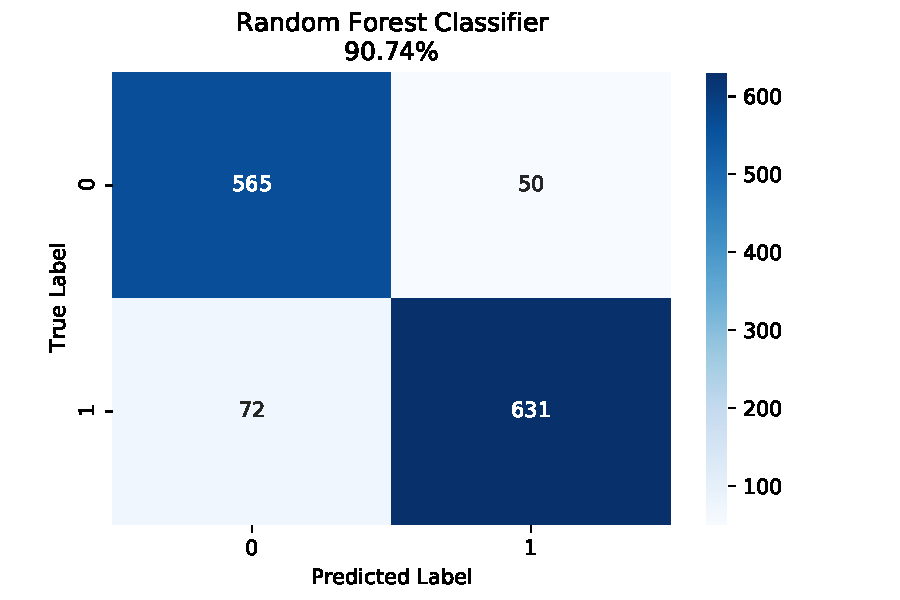
\includegraphics[width = 0.23\textwidth]{figures/j_rfc}
	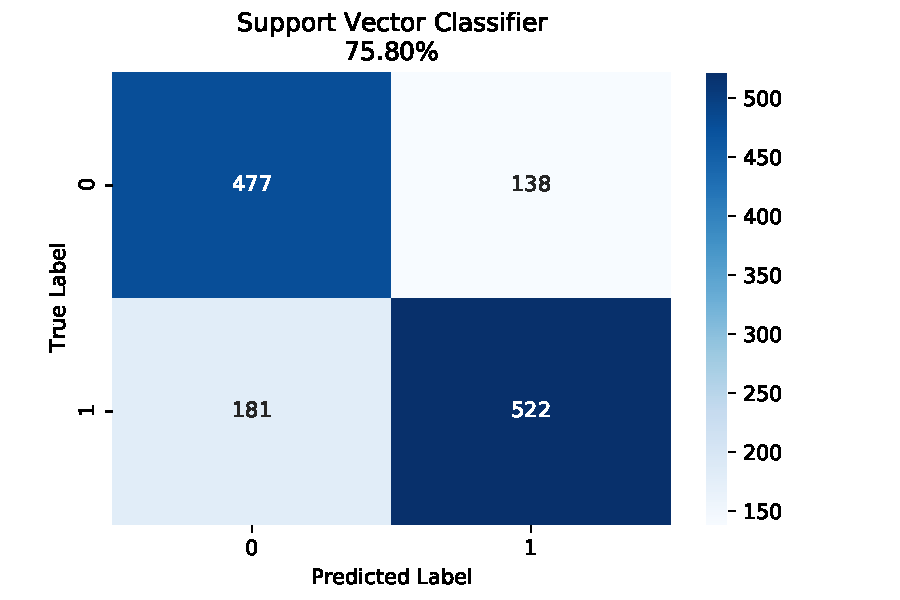
\includegraphics[width = 0.23\textwidth]{figures/j_svc}
	\caption{Confusion matrices for different classification algorithms trained on the Jarvis dataset.}
	\label{fig:j}
\end{figure}

\begin{table}[]
\centering
\caption{Comparison of performance of various regression algorithms on eight-dimensional C2DB and JARVIS.}
\label{tab:only}
\begin{tabular}{@{}ccccccc@{}}
\toprule
\multicolumn{1}{l}{} & \multicolumn{1}{l}{} & C2DB & \multicolumn{1}{l}{} & \multicolumn{1}{l}{} & JARVIS & \multicolumn{1}{l}{} \\ \midrule
\multicolumn{1}{l}{} & $R^2$                & MAE  & RMSE                 & $R^2$                & MAE    & RMSE                 \\
SVR                  & 0.73                 & 0.24  & 0.41                 & 0.74                 & 0.46   & 0.81                 \\
RF                   & 0.90                 & 0.10  & 0.25                & 0.82                 & 0.88   & 1.28                 \\
GBDT                 & 0.91                 & 0.09 & 0.24                 & 0.77                 & 0.38   & 0.75                 \\ \bottomrule
\end{tabular}
\end{table}

We built ML models for three purposes, classification, regression and clustering. In the following subsections we briefly describe the mode of implementation of these algorithms and the need to implement them. All the ML algorithms are implemented using scikit-learn [11] Python library with default values of model parameters unless mentioned otherwise. \href{https://github.com/SagarPrakashBarad/ML-EBGEstimate}{Github link to the project repository}.

\subsection{Classification}

We built a classifier to classify between metals and non-metals. We labelled the data on the basis of band gap values. Materials with band gap equal to zero were labelled as metals. We built this classifier with the aim of eliminating metals quickly. We used four classification algorithms, support vector classification, logistic regression, decision tree classification and random forest classification. The confusion matrix for each of the algorithm obtained on both the datasets in present in figures \ref{fig:c} and \ref{fig:j}. The random forest classifier performed the best in both the datasets. In the \emph{LogisticRegression} function we changed the \emph{max\_iter} argument to \emph{999999999} and in the \emph{SVC} function we changed the \emph{probability} argument to \emph{True}, for both the datasets. 

\subsection{Regression}

We use three regression algorithms for predicting the band gap, support vector regression, random forest and gradient boosted decision trees. The performance of the different models on both the datasets in shown in table \ref{tab:only}. For all the three algorithms we used the model parameters used by Zhang et al. [1].

\subsection{Ensemble Methods}

We used stacked generalisation method in an attempt to achieve a higher $R^2$ value. We performed two experiments and in both the experiments ended up with a worse $R^2$ value. We only applied these methods on C2DB. In both the experiments random forest regressor is used as the final estimator. In the first experiment we use all the three algorithms that we used to train C2DB with same values of the parameters, we achieved $R^2 = 0.78$. While in the second experiment we dropped the support vector regressor from the first layer, and achieved $R^2 = 0.77$

\subsection{Clustering}

We used DBSCAN for clustering the datasets. While clustering we removed the band gap value from the features. In future we want to train ML models on these clusters separately. For C2DB dataset we got $7$ clusters with zero noise points with \emph{eps = 120} and \emph{min\_samples = 1} while for JARVIS we got $6$ clusters with \emph{eps = 100} and \emph{min\_samples = 3}.

\section{Future Plans}

Following are some of our future plans:
\begin{enumerate}
	\item Improve the ensemble methods and train them on the clusters obtained through DBSCAN.
	\item Further improve the metal non-metal classifier through ensemble methods. 
	\item Explore encoding methods to enable better learning of material properties Rosen et al. [5].
	\item Train deep learning networks on bigger datasets such as Materials Project and AFLOW Dong et al. [2].
	\item Explore the use of graph neural networks and representation learning in learning materials properties Yan et al. [8]. 
\end{enumerate}

\newpage

\section*{References}


{
\small


[1] Zhang Y, Xu W, Liu G, Zhang Z, Zhu J, \ \& Li M (2021) {\it Bandgap prediction of two-dimensional materials using machine learning.} {\it PLoS ONE} 16(8): e0255637. \url{https://doi.org/10.1371/journal.pone.0255637}


[2] Dong Y., Wu C., Zhang C., Liu Y., Cheng J., \ \& Lin J. (2019) {\it Bandgap prediction by deep learning in configurationally
hybridized graphene and boron nitride.} {\it npj Computational Materials} 5:26. \url{https://doi.org/10.1038/s41524-019-0165-4}


[3] Olsthroon B., Geilhufe M. R., Borysov S. S. \ \& Balatsky A. V. (2019) {Band gap prediction for large organic crystal structures with machine learning.} {\it Advanced Quantum Technologies} Volume 2, Issue 7-8. \url{https://doi.org/10.1002/qute.201900023}

[4] Gao C., Yang X., Jiang M., Chen L., Chen Z., \ \& Singh V. C. (2022) {\it Machine learning-enabled band gap prediction of monolayer transition metal chalcogenide alloys.} {\it Phys. Chem. Chem. Phys.} {\bf 24}, 4653. \url{10.1039/d1cp05847a}

[5] Rosen I., Qu J., \ \& Marks J. (2018) {\it Predicting electronic properties of materials.} {\it CS229 Report}.

[6] Hayee F. \ \& Datye I. {\it Data-driven prediction of band gap of materials.} {\it CS229 Report}.

[7] Kauwe, S.K., Welker, T. \ \& Sparks, T.D. {\it Extracting Knowledge from DFT: Experimental Band Gap Predictions Through Ensemble Learning.} {\it Integr Mater Manuf Innov 9}, 213–220 (2020). \url{https://doi.org/10.1007/s40192-020-00178-0}

[8] Yan K., Liu Y., Lin Y., \ \& Ji S. (2022) {\it Periodic graph transformers for crystal material property prediction.} {\it 36th Conference on Neural Information Processing Systems (NeurIPS 2022).} 

[9] Zhuo Y., Tehrani A. M., \ \& Brgoch J. (2018) {\it Predicting the band gaps of inorganic solids by machine learning.} {\it The Journal of Physical Chemistry Letters} 9, 1668-1673. \url{10.1021/acs.jpclett.8b00124}

[10] Carleo G., Cirac I., Cranmer K., Daudet L., Schuld M., Tishby N., Vogt-Maranto L., \ \& Zdeborová L. (2019) {\it Machine learning and the physical sciences.} {\it Reviews of Modern Physics} 91, 045002. \url {10.1103/RevModPhys.91.045002}

[11] Pedregosa, F., Varoquaux, G., Gramfort, A., Michel, V., Thirion, B., Grisel, O., Blondel, M., Prettenhofer, P., Weiss, R., Dubourg, V., Vanderplas, J., Passos, A., Cournapeau, D., Brucher, M., Perrot, M. \ \& Duchesnay, E. (2011) {\it Scikit-learn: Machine Learning in Python.} {\it Journal of Machine Learning Research} 12, 2825--2830. \url{https://scikit-learn.org/stable/index.html}

[12] Choudhary, K., Singh, A., Ghosh, S., Zhang, F., \ \& Srinivasan, S.\  (2020). The joint automated repository for various integrated simulations (JARVIS) for data-driven materials design. {\it G. Tesauro, D.S. Touretzky, \& T.K. Leen (Eds.), Advances in Neural Information Processing Systems 7 (pp. 609-616). npj Computational Materials}.

[13] Haastrup, S.,  Strange, M., Pandey, M., Deilmann, T., Schmidt, S., Hinsche, .N, Gjerding, M.N ., Torelli, D., Larsen, P.M., Riis-Jensen, A.C.,  Gath, J., Jacobsen, K.W, Mortensen, J.J., Olsen T., \  \& Thygesen, K.S.\  (2018). The Computational 2D Materials Database: High-Throughput Modeling and Discovery of Atomically Thin Crystals.{\it  2D Materials}, (5)(4), 042002.

}



\end{document}
